\documentclass[12pt,openright,twoside,french]{book}

\input philippe2013
\input philippe2013_activites

\geometry{a4paper, height = 26.5cm,hmargin=1.5cm,marginparwidth=2cm,headheight=20pt,headsep=16.5pt,bottom=2cm,footskip=30pt,footnotesep=30pt}

\pagestyle{empty}

\begin{document}
\small

\TitreExo{\bsc{ix}.1}{Fonctions circulaires \\ Applications}

\textbf{Propriété :} La période de la fonction $t \mapsto A \times \cos(\omega t + \varphi)$ est égale à $\dfrac{2\pi}{\omega}$.\[*\]

\textbf{\'Etude d'un signal électrique : exercice 38 page 149}

On réalise un montage électrique permettant d'entretenir des oscillations sinusoïdales et on obtient sur un oscilloscope cathodique la courbe suivante pour la tension :
\[u(t) = U_m \times \cos(\omega t).\]

\begin{center}
    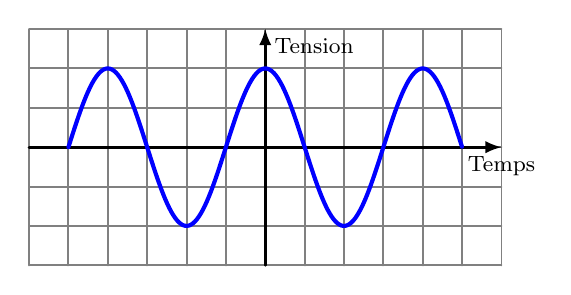
\begin{tikzpicture}[line cap=round,line join=round,>=latex,y=0.1cm,x=1cm]
        \footnotesize
        \draw [color=gray, xstep=0.5,ystep=5,line width=0.7pt] (-3,-15) grid (3,15);
        \draw[->,line width=1pt] (-3,0) -- (3,0) node[below] {Temps};
        \draw[->,line width=1pt] (0,-15) -- (0,15) node [below right] {Tension};
        \draw[blue,line width = 1.5pt,domain=-2.5:2.5,samples=200]plot(\x,{10*cos(deg(pi*\x))});
    \end{tikzpicture}
\end{center}

\begin{enumerate}
    \item Sachant qu'une division horizontale correspond à $0.5~ms$, déterminer graphiquement la période de la fonction $u$.
    \item En utilisant la propriété en haut de la feuille, en déduire alors la valeur de $\omega$ exprimée en $ms^{-1}$.
    \item Sachant qu'une division verticale correspond à $5~V$, déterminer graphiquement la tension à l'instant $t = 0$.
    \item Déduire alors du calcul de $u(0)$ la valeur de la constante $U_m$ exprimée en Volts.
    \item Déduire des questions précédentes l'expression de $u(t)$, en Volts, en fonction de $t$, en millisecondes.
    \item Dresser le tableau de variations de la fonction $u$ sur l'intervalle $\intervalleff{0}{2,5}$.
\end{enumerate}\[*\]

\textbf{\'Etude de fonctions}

\begin{enumerate}
    \item Soit la fonction $f$ définie sur $\R$ par $f(t) = 4\cos(4t)$.
        \begin{enumerate}
            \item Représenter la courbe de $f$ sur la calculatrice. Quel semble être le maximum ?
            \item Montrer que $f$ est paire.
            \item Montrer que $f$ est $\dfrac{\pi}{2}$-périodique.
            \item \'Etablir le tableau de variation de $f$ sur $\intervalleff{0}{\dfrac{\pi}{4}}$.
            \item En choisissant $6$ carreaux pour $\pi$ en abscisses, tracer la courbe de la fonction $f$ sur $\intervalleff{0}{\dfrac{\pi}{4}}$ puis compléter cette courbe sur $\intervalleff{-\dfrac{\pi}{4}}{\dfrac \pi 4}$ et enfin sur $\intervalleff{-2\pi}{2\pi}$.
        \end{enumerate}
    \item On rappelle que $\cos(x) = \sin\left(x + \dfrac\pi 2\right)$.
        \begin{enumerate}
            \item On considère la fonction $h$ définie sur $\R$ par $h(t) = 4\sin\left(4t - \dfrac\pi 3\right)$. \'Ecrire $h$ en fonction de $f$.
            \item En déduire la translation qui permet de passer de la courbe de $f$ à celle de $h$.
            \item Sur le graphique précédent, tracer la courbe de $h$.
        \end{enumerate}
\end{enumerate}

\end{document} 